\section{Code}

I have implemented two examples using the \textit{KAN} library to demonstrate where KANs are particularly useful, not only on toy datasets. 
\newline
\textbf{Link:} \url{https://github.com/matteopasqual02/KAN-naml/blob/master/KANs_code.ipynb}

The first example is a regression task on a non-linear function. The focus is on achieving high accuracy, demonstrating pruning efficiency, ensuring interpretability, and showcasing how automatic symbolic regression can generate the optimal model.

The second example involves a classification task on the cancer dataset from \texttt{sklearn}. This example highlights the practical value of KANs when applied to a real-world dataset.

\subsection{Regression}

The regression task involves training a Kolmogorov Arnold Network (KAN) to learn the non-linear function \( f(x, y) = e^{\sin(\pi x) + y^2} \). Below are the main steps and highlights of the task:

\begin{itemize}
    \item \textbf{Network Architecture:}
    \begin{itemize}
        \item Three layers: input layer (2 neurons), hidden layer (5 neurons), output layer (1 neuron).
        \item Cubic splines (degree 3) are used as activation functions in the hidden layer.
        \item Input space is divided into five grid intervals.
    \end{itemize}

    \item \textbf{Dataset:}
    \begin{itemize}
        \item Synthetic dataset generated using the target function \( f(x, y) \).
        \item Inputs are normalized, and the dataset is split into training and test sets.
    \end{itemize}

    \item \textbf{Training Process:}
    \begin{itemize}
        \item Optimization algorithm: L-BFGS, a second-order optimization method.
        \item Training duration: 50 iterations.
        \item Regularization: Sparsity (\( \lambda = 0.01 \)) and  Entropy (\( \lambda_{\text{entropy}} = 10 \))  regularization.
        
    \end{itemize}

    \item \textbf{Pruning:}
    \begin{itemize}
        \item The KAN is pruned to eliminate redundant components, simplifying its structure.
        \item The network is retrained post-pruning to improve accuracy.
    \end{itemize}

    \item \textbf{Symbolic Regression:}
    \begin{itemize}
        \item A symbolic representation of the learned function is derived using a library of functions.
        \item This step emphasizes the model's interpretability while retaining high accuracy.
    \end{itemize}
\end{itemize}

\subsubsection{Experimental Results}
The KAN approximates the target function with high accuracy. Therefore, pruning and symbolic regression enhance the model's sparsity and interpretability, making it efficient and explainable.
The obtained accuracies after symbolic regression are as follows:
\begin{itemize}
    \item \textbf{Training Accuracy:} 1.0
    \item \textbf{Test Accuracy:} 1.0
\end{itemize}

\begin{figure}[H]
    \centering
    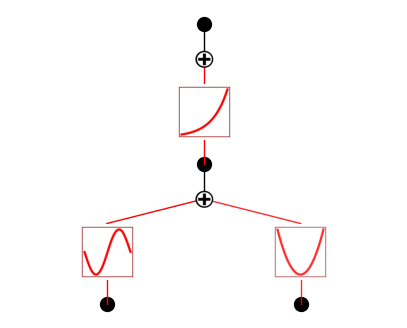
\includegraphics[width=0.35\linewidth]{LATEX//Images/symbolic.png}
    \caption{Network structure after pruning}
    \label{fig:sy}
\end{figure}

Figure \ref{fig:reg} illustrates how symbolic regression resulted in perfect accuracy, while Figure \ref{fig:sy} demonstrates the high interpretability of the network.

\begin{figure}[H]
    \centering
    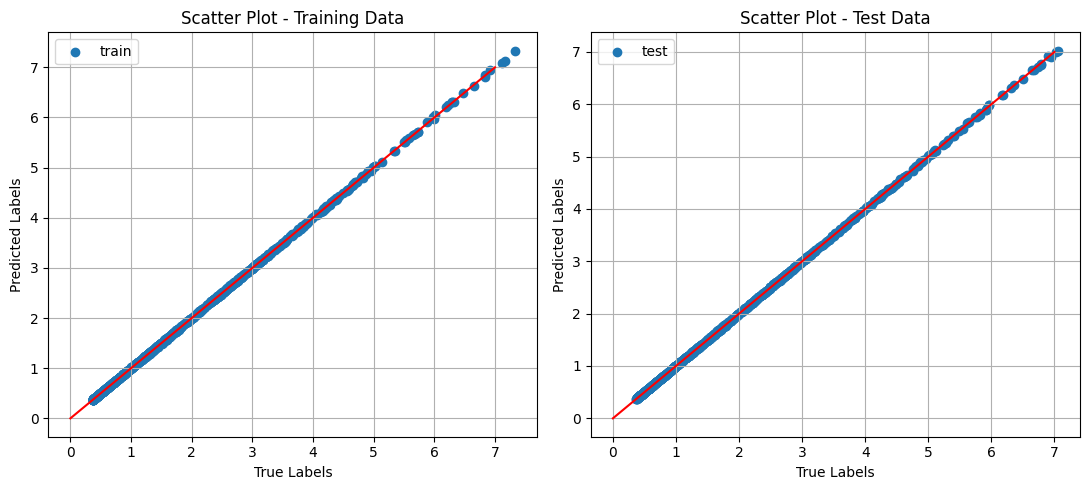
\includegraphics[width=0.75\linewidth]{LATEX//Images/regression.png}
    \caption{Symbolic regression results}
    \label{fig:reg}
\end{figure}




\subsection{Cancer analisys}

The cancer analysis task involves training a Kolmogorov Arnold Networks (KAN) to predict outcomes based on clinical and pathological data. Below are the main steps and highlights of the analysis:

\begin{itemize}
    \item \textbf{Dataset:}
    \begin{itemize}
        \item The Wisconsin Breast Cancer Dataset is used, containing 569 samples and 30 features.
        \item The dataset is normalized and split into training and test sets.
    \end{itemize}

    \item \textbf{Network Architecture:}
    \begin{itemize}
        \item Three layers: input layer (30 neurons), hidden layer (10 neurons), output layer (1 neuron).
        \item Cubic splines (degree 3) are employed as activation functions.
        \item Input space is divided into 10 grid intervals.
    \end{itemize}

    \item \textbf{Training Process:}
    \begin{itemize}
        \item Optimization algorithm: L-BFGS, a second-order optimization method.
        \item Regularization techniques include:
        \begin{itemize}
            \item Sparsity regularization (\( \lambda = 0.05 \)).
            \item Entropy regularization (\( \lambda_{\text{entropy}} = 5 \)).
        \end{itemize}
    \end{itemize}

    \item \textbf{Model Evaluation:}
    \begin{itemize}
        \item Accuracy, precision, recall, and F1-score are used as evaluation metrics.
        \item Confusion matrices are plotted to visualize TP, TN, FP, and FN.
    \end{itemize}

    \item \textbf{Pruning:}
    \begin{itemize}
        \item The KAN is pruned to remove redundant components, simplifying its structure.
        \item The network is retrained post-pruning to improve efficiency without sacrificing accuracy.
    \end{itemize}

    \item \textbf{Symbolic Regression:}
    \begin{itemize}
        \item A symbolic representation of the predictive model is derived.
        \item In this dataset, symbolic regression isn't useful since there isn't a real formula in the data.
    \end{itemize}

    \item \textbf{Results:}
    \begin{itemize}
        \item The KAN achieves high classification accuracy on the test set.
        \item Pruning improves the model's accuracy and interpretability.
    \end{itemize}

\end{itemize}

\subsubsection{Experimental Results}
The obtained accuracies are as follows:
\begin{itemize}
    \item \textbf{Training Accuracy:} 0.978
    \item \textbf{Test Accuracy:} 0.974
\end{itemize}

The Figure\ref{fig:CM} shows the confusion matrix for both datasets::

\begin{figure}[H]
    \centering
    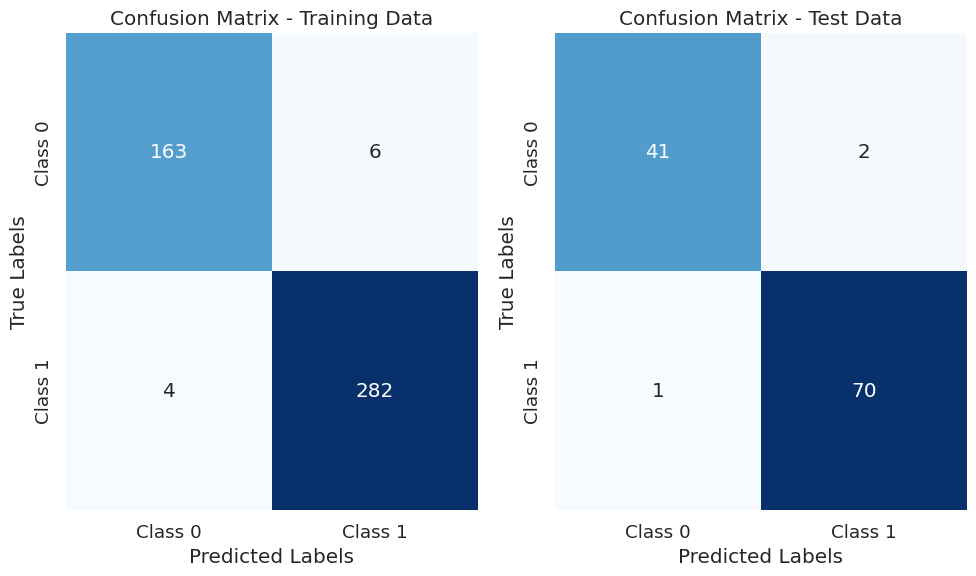
\includegraphics[width=0.65\linewidth]{LATEX//Images/CMcancer-pruning.png}
    \caption{Confusion Matrix for Cancer Analysis after Pruning}
    \label{fig:CM}
\end{figure}